\section{Conjuntos, relaciones y funciones}
\subsection{Conjuntos}
\paragraph{Conjunto:} Es una colección de objetos tales que, dado un objeto cualquiera $v$, se puede determinar si $v$ pertenece o no a la misma.

\paragraph{Conjunto vació:} 
Es el conjunto que no tiene elementos  y se lo denota con la letra $\phi$.

\paragraph{Cardinal:} 
de un conjunto $A$ es el número de elementos distintos que posee el mismo y lo notamos $|A|$.
    
\paragraph{Subconjunto:} 
Se dice que un conjunto $B$ está contenido en un conjunto $A$ si todo elemento de $B$ es un elemento de $A$.
    \begin{align*}
        B\subseteq A\iff[(\forall~x:\alpha)~x\in B \to x\in A]
    \end{align*}
    
\paragraph{Igualdad: }
Dos conjuntos $A$ y $B$ son iguales si tienen exactamente los mismos elementos.
    \begin{equation*}
        A = B \iff (A\subseteq B \land B\subseteq A)
    \end{equation*}
    
\paragraph{Conjunto referencial: }
Conjunto que incluye a todos los conjuntos que se están considerando. Sean $A$ y $B$ dos conjuntos cualesquiera:
        \begin{center}
         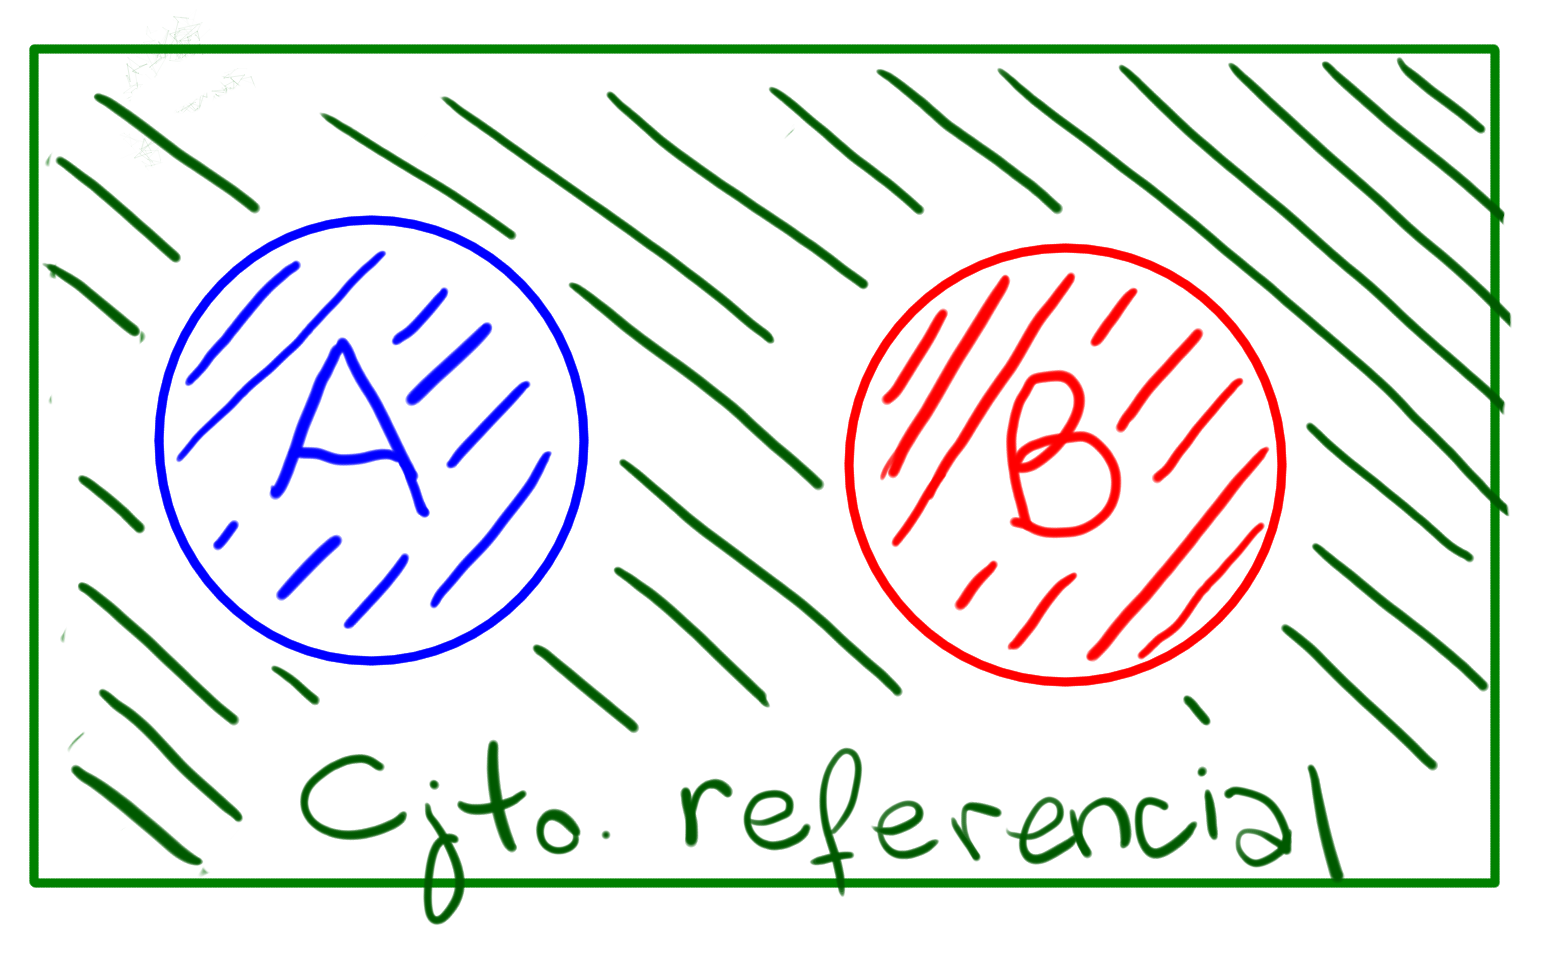
\includegraphics[scale=0.3]{imagenes/cjto_referencial.png}
        \end{center}
        
\paragraph{Complemento: }
Sea $A\subset U$ entonces, el complemento $A^c$ de $A$ es el conjunto que incluye todos los elementos de $U$ que no pertenecen a $A$.
    \begin{center}
    \begin{minipage}{0.3\textwidth}
        \begin{equation*}
            A^c = \{x\in U : x\notin A\}
        \end{equation*}
    \end{minipage}
    \begin{minipage}{0.4\textwidth}
         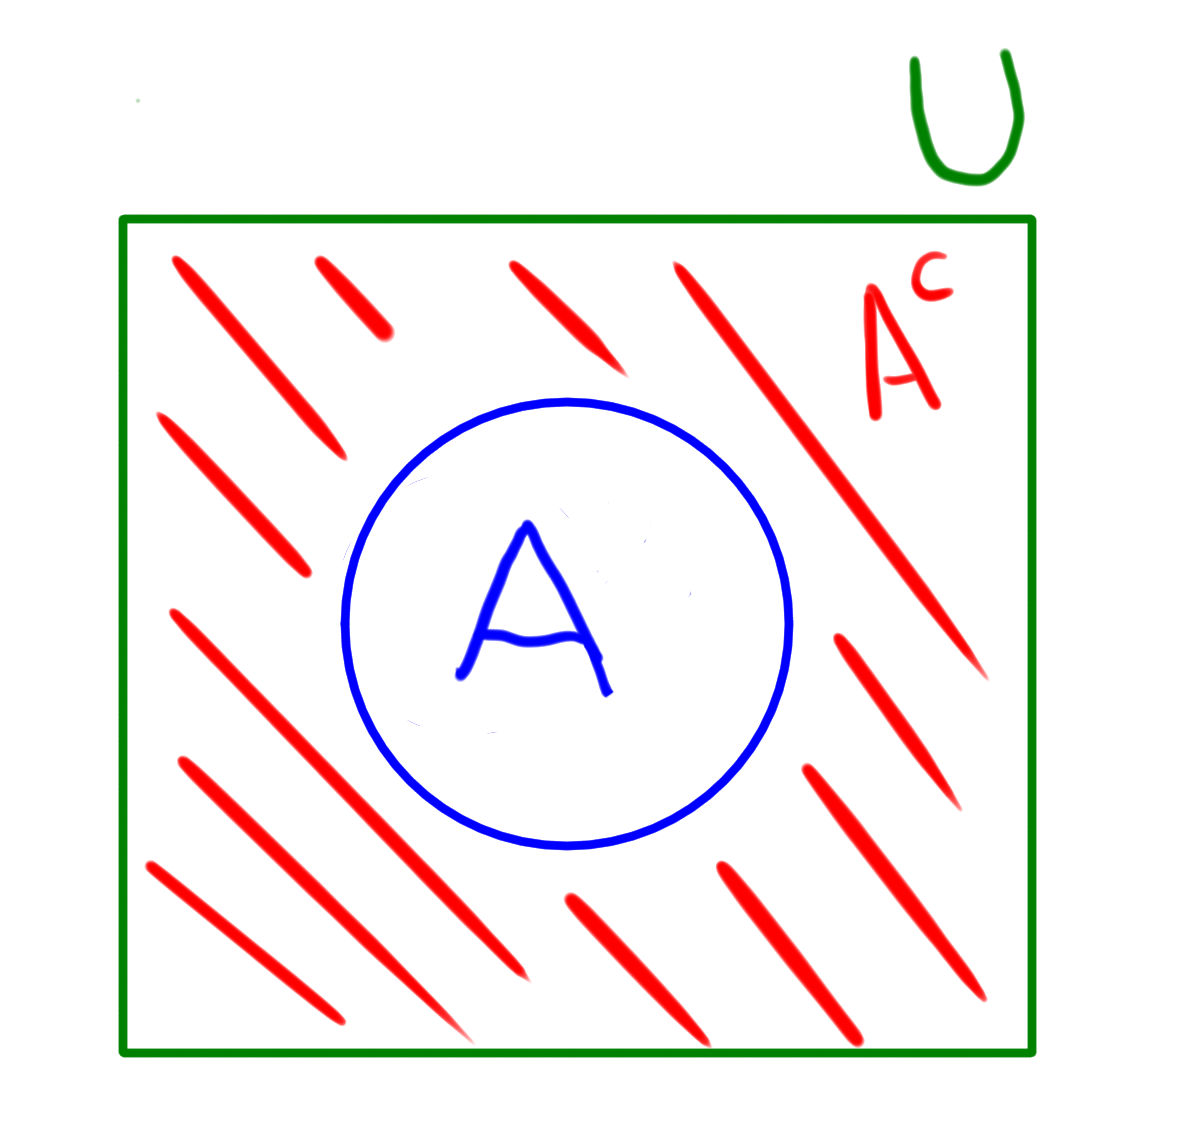
\includegraphics[scale=0.3]{imagenes/complemento.png}
    \end{minipage}
    \end{center}
    
\paragraph{Intersección: }
Sean $A\subset U$ y $B\subset U$, la intersección de $A$ y $B$ es el cojunto de elementos que pertenecen tanto a $A$ como a $B$.
        \begin{center}
    \begin{minipage}{0.4\textwidth}
        \begin{equation*}
            A\cap B = \{x\in U : x\in A \land x\in B\}
        \end{equation*}
    \end{minipage}
    \begin{minipage}{0.4\textwidth}
         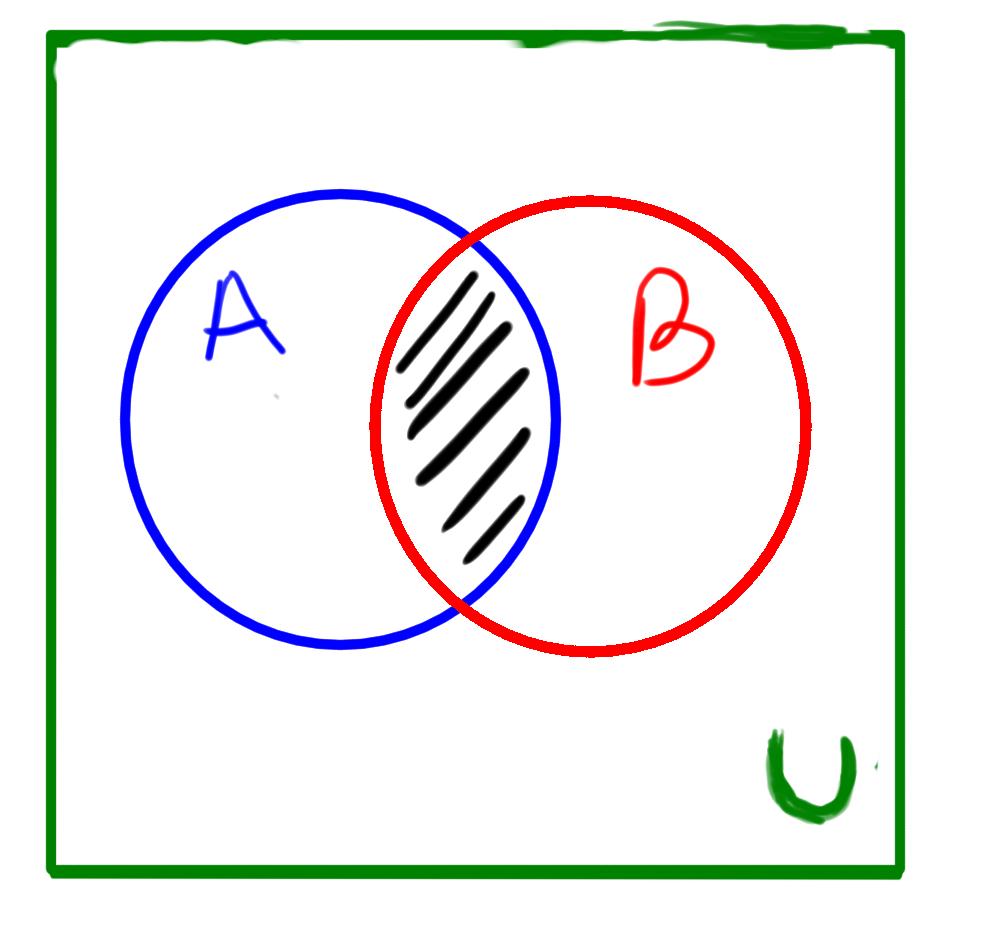
\includegraphics[scale=0.3]{imagenes/intersection.png}
    \end{minipage}
    \end{center}
    
\paragraph{Union:}
Sean $A\subset U$ y $B\subset U$, la \textbf{union} de $A$ y $B$ es el conjunto de elementos que pertenecen a $A$ o a $B$.
        \begin{center}
    \begin{minipage}{0.4\textwidth}
        \begin{equation*}
            A\cup B = \{x\in U : x\in A \lor x\in B\}
        \end{equation*}
    \end{minipage}
    \begin{minipage}{0.4\textwidth}
         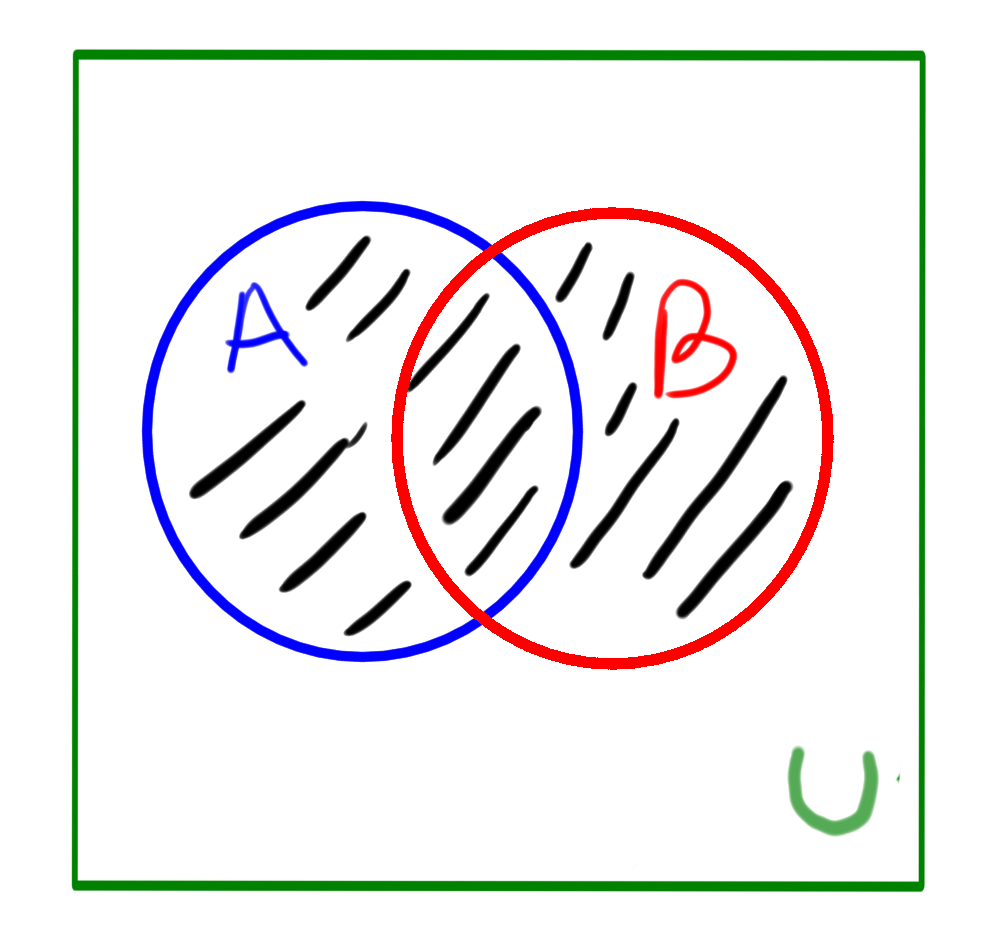
\includegraphics[scale=0.3]{imagenes/union.png}
    \end{minipage}
    \end{center}

\paragraph{Propiedades}
  \begin{itemize}    
    \item $\phi$ está contenido en todos los conjuntos.
    \item Sean $A$ y $B$ dos conjuntos tal que $B\subseteq A \to |B|\leq|A|$
    \begin{multicols}{2}
        \item Si $A\cap B = \phi \to |A\cup B|  = |A| + |B|$
        \item $|A\cup B| = |A| + |B| - |A\cap B|$
        \item Si $U$ es finito, $|A^c| = |U|-|A|$
        \item Si $A\subseteq B \land B\subseteq C$ entonces $A\subseteq C$
        \item Si $A\subseteq B \land A\subseteq C$ entonces $A \subseteq (B\cap C)$
        \item $A\subseteq (A\cup B) \land B\subseteq (B\cup A) \to A = B$
        \item $A\cap(B\cap C) = (A\cap B)\cap C$
        \item $A\cap B = B\cap A$
        \item $A\cap A^c = \phi$
        \item $A\cap\phi=\phi$
        \item $A\cup(B\cup C) = (A\cup B)\cup C$
        \item $A\cup B = B\cup A$
        \item $A \cup A^c = U$
        \item $A\cup\phi=A$
    \end{multicols}
\end{itemize}

\paragraph{Leyes de Morgan:} 
Sean $A$ y $B$ contenidos en $U$, entonces valen:
    \begin{itemize}
    \begin{multicols}{2}
    \item $(A\cup B)^c = A^c\cap B^c$
        \item $(A\cap B)^c = A^c\cup B^c$
    \end{multicols}
    \end{itemize}

\paragraph{Diferencia: }
Sean $A\subset U$ y $B\subset U$, la diferencia entre $A$ y $B$ se define como:
        \begin{center}
    \begin{minipage}{0.4\textwidth}
        \begin{align*}
            A - B &= A \cap B^c \\ &= \{x\in U : x\in A \land x\notin B\}
        \end{align*}
    \end{minipage}
    \begin{minipage}{0.4\textwidth}
         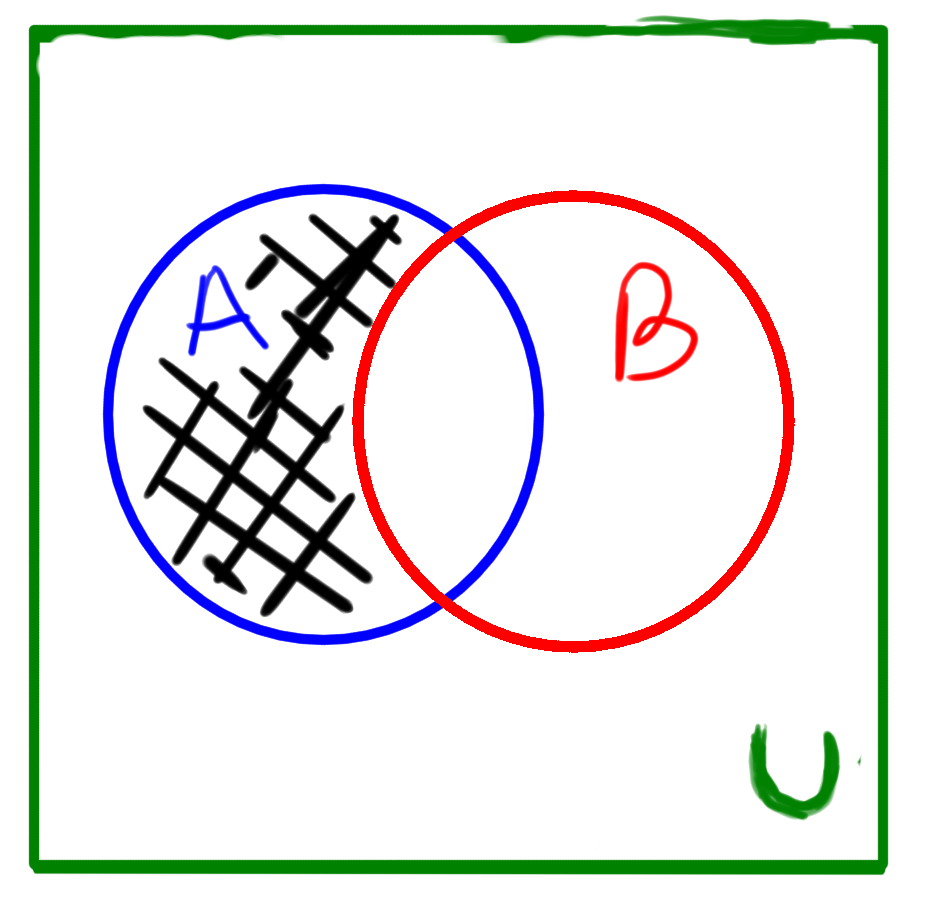
\includegraphics[scale=0.3]{imagenes/difference.png}
    \end{minipage}
    \end{center}
    
\paragraph{Propiedades:}
    \begin{itemize}
    \begin{multicols}{2}
    \item $A - B = A - (A\cap B)$
    \item $|A-B| = |A| - |A\cap B|$    
    \end{multicols}
    \end{itemize}
    
\paragraph{Diferencia simétrica:} Sean $A\subset U$ y $B\subset U$, la diferencia simétrica entre $A$ y $B$ es el conjunto de elementos que pertenecen a $A$ o a $B$ pero no los dos a la vez.
        \begin{center}
    \begin{minipage}{0.4\textwidth}
        \begin{align*}
            A \triangle B &= (A-B)\cup(B-A)
        \end{align*}
    \end{minipage}
    \begin{minipage}{0.4\textwidth}
         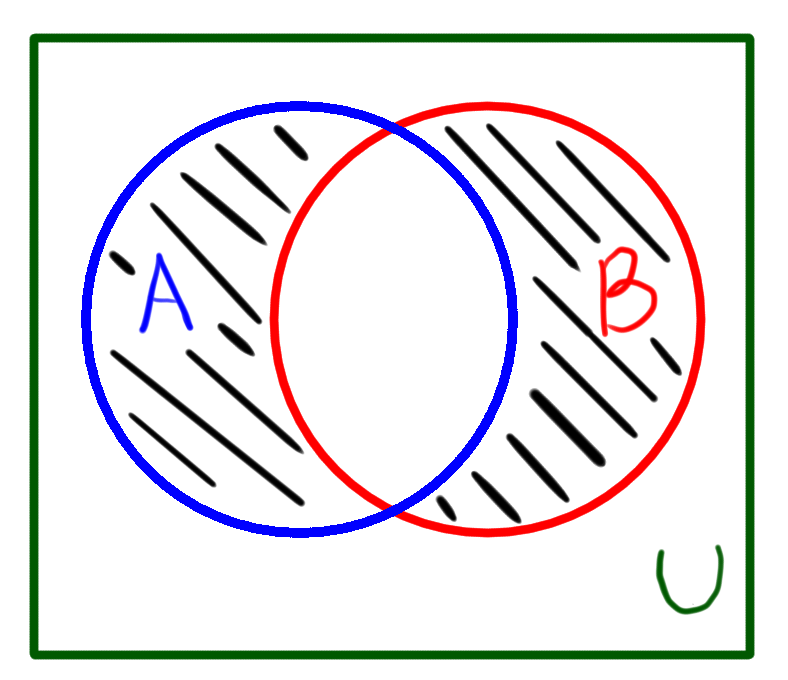
\includegraphics[scale=0.3]{imagenes/symetrical_difference.png}
    \end{minipage}
    \end{center}
    
\paragraph{Propiedades:} Sean $A$, $B$ y $C$ subconjuntos de $U$:
        \begin{itemize}
    \begin{multicols}{2}
    \item $|A\triangle B| = |A| + |B| - 2\times|A\cap B|$        
        \item $A\triangle B = (A\cup B) - (A\cap B)$
        \item $A\triangle B = B\triangle A$
        \item $A\triangle A = \phi$
        \item $A\triangle\phi = A$
        \item $(A\triangle B) - C = (A - C)\triangle (B-C)$
        \item $(A\triangle B)\subseteq (A\triangle C)$
        \end{multicols}
    \end{itemize}
    
\paragraph{Conjunto de partes:} de $A$ se nota $\partes(A)$ y es el conjunto formado por todos los subconjuntos de $A$.
    \begin{equation*}
        \partes(A) = \{B : B\subseteq A\}\land 
        (B\in \partes(A)\iff B\subseteq A)
    \end{equation*}
    
\paragraph{Propiedades}:
    \begin{itemize}
    \begin{multicols}{2}
        \item $\partes(A) \subseteq \partes(B) \iff A\subseteq B$
        \item $|\partes(A)| = 2^{|A|}$
    \end{multicols}
        
    \end{itemize}
    
\paragraph{Producto cartesiano} Sean $A$ y $B$ conjuntos, el producto cartesiano de $A$ con $B$ es el conjunto de pares ordenados $A\times B = \{(x,y) : x\in A \land y \in B\}$

\paragraph{Propiedades:}
    \begin{itemize}
        \item $|A\times B| = |A||B|$
        \item $|A_1\times\dots\times A_n| = |A_1|\times\dots\times|A_n|$ 
        \item $A\neq B$ entonces $A\times B \neq B\times A$
        \item Si $A\subseteq U \land B\subseteq V$ entonces $A\times B \subseteq U\times V$
    \end{itemize}
    


\subsection{Relaciones}
    Sean $A$ y $B$ dos conjuntos. Un subconjunto $\rel$ del producto cartesiano $A\times B$ se llama relación de $A$ en $B$.
    
    Dados $x\in A$ e $y\in B$ y una relación $\rel$ de $A$ en $B$, se dice que $x$ esta relacionado con $y$ si $(x,y)\in\rel$. Y, en ese caso, se nota $x\rel y$.
    
    Se dice que $\rel$ es una relación en $A$ cuando $\rel\subseteq A\times A$. Una relación $\rel$ en $A$ puede ser:
    
    \begin{itemize}
        \item \textbf{Reflexiva:} si $(\forall~ x\in A)~(x,x)\in\rel $
        \item \textbf{Simétrica:} si $(\forall~ x,y\in A)~(x\rel y \to y\rel x)$
        \item \textbf{Asimétrica:} si $(\forall~ x,y\in A)~(x\rel y \land y\rel x \to x = y)$.
        \item \textbf{Transitiva}: Si $(\forall~ x,y,z\in A)~(x\rel y \land y\rel z \to x\rel z)$.
    \end{itemize}
    
\subsubsection{Relaciones de equivalencia y de orden}
    $\rel$ es una \textbf{relación de equivalencia} si es reflexiva, simétrica y transitiva.
    
    $\rel$ es una \textbf{relación de orden} cuando es una relación reflexiva, asimétrica y transitiva.
        
    Dada $\sim$ una relación de equivalencia en $A$, la \textbf{clase de equivalencia} de un elemento $x\in A$, es el conjunto $C_x = \overline{x} = \{y\in A: y\sim x\}$
        
    \begin{itemize}
        \item Si $y\in C_x$ entonces $x\in C_y$
        \item $x\in C_x$
        \item $x\sim y \iff C_x = C_y$
        \item $x\not\sim y \iff C_x \cap C_y = \phi$
    \end{itemize}    
    
\subsubsection{Partición de un conjunto}
    Sea $A$ un conjunto y $\partes$ un conjunto formado por subconjuntos de $A$. Decimos que $\partes$ es una \textbf{partición} si cumple:
    
    \begin{itemize}
        \item $\partes\neq\phi$
        \item Si $P, Q \in \partes \land P\neq Q$ entonces $P\cap Q = \phi$
        \item Para todo elemento $a$ de $A$, $(\exists~ P\in\partes)~a\in P$
    \end{itemize}
    
    Para todo conjunto $A$, hay una manera natural de asociar una relación de equivalencia en $A$ a una partición de $A$. 
        
    Sea $\sim$ una relación de equivalencia en un conjunto $A$:
    
    \begin{itemize}
        \item Sean $a,b\in A$, entonces $a\sim b \iff$ existe $c\in A$ tal que $a,b\in C_c$.
        \item $\partes = \{C_a : a\in A\}$ es una partición de $A$.
    \end{itemize} 
    
    Si $\partes$ es una partición de $A$, entonces la relación $\sim$ en $A$ definida por ''$a\sim b \iff \exists~P\in\partes$ tal que $a,b\in P$'' es de equivalencia.

    Si $A$ y $B$ son conjuntos finitos con $m$ y $n$ elementos, respectivamente, entonces, la cantidad de relaciones que hay de $A$ en $B$ es igual a $2^{mn}$    
    \subsection{Funciones}
    Dada $f$ una relación de $A$ en $B$, se dice que $f$ es una \textbf{función} cuando todo elemento $x\in A$ está relacionado con algún elemento $y\in B$ y además es el único elemento con el que se relaciona. Si pasa esto, se dice que $y$ es la imagen de $x$ por $f$ ($y=f(x)$).
    
    La $\rel = \{(x,x) : x\in A\}$ para cualquier conjunto $A\neq\phi$, es la \textbf{función identidad} de $A$ y se nota $id_A$.  ($id_A(x) = x ~\forall x\in A$)
    
    Si $A$ es un conjunto, una sucesión de elementos de $A$ puede ser tomada como una función $f:\nat\to A$.
    
    Sean $f,\func{g}{A}{B}$, $f$ y $g$ son \textbf{iguales} ($f=g$) cuando $f(x) = g(x)~\forall~x\in A$
    
    Sea $\func{f}{A}{B}$:
    \begin{itemize}
        \item $A$ se llama \textbf{dominio} de $f$
        \item $B$ se llama \textbf{codominio} de $f$
        \item La \textbf{imagen} $\texttt{Im}(f)$ es el subconjunto de elementos de $B$ que están relacionados con algún elemento de $A$
        \begin{equation*}
            \texttt{Im}(f) = \{y\in B : \exists~x\in A / f(x) = y\}
        \end{equation*}
        \item $f$ es \textbf{inyectiva} si $\forall~y\in B$ existe a lo sumo un elemento $x\in A / f(x) = y$
        \item $f$ es \textbf{sobreyectiva} si $\forall~y\in B$ existe al menos un elemento de $x\in A / f(x)=y$.
        \item $f$ es \textbf{biyectiva} si es inyectiva y sobreyectiva.
    \end{itemize}
    
     
    Sean $A$ y $B$ dos conjuntos de $m$ y $n$ elementos respectivamente, entonces hay $n^m$ funciones de $A$ en $B$ distintas y dada una función $\func{f}{A}{B}$ vale que:
    \begin{itemize}
        \item Si $f$ es inyectiva $\to |A|\leq|B|$
        \item Si $f$ es sobreyectiva $\to|A|\geq|B|$
        \item Si $f$ es biyectiva $\to|A|=|B|$
    \end{itemize}
    
    Además hay $n!$ funciones biyectivas de $A$ en $B$ y $\frac{n!}{(m-n)!}$ funciones inyectivas de $A$ en $B$.
    
    \subsubsection{Composición de funciones y función inversa}
    Sean $\func{f}{A}{B}$ y $\func{g}{B}{C}$ funciones, entonces la \textbf{composición} $g\circ f$ de $f$ con $g$ está definidad por:
    \begin{equation*}
        \comp{g}{f}{A}{C},~(g\circ f)(x) =g(f(x))
    \end{equation*}

    Si $f$ es una función biyectiva, entonces para todo $y\in B$ existe exactamente un elemento $x\in A / f(x)=y$. Sea $\rel=\{(y,x) : f(x)=y\}$ una relación de $A$ en $B$, se puede ver que $\rel$ satisface las propiedades para ser función. Notamos $\rel$ con $f^{-1}$ y se llama \textbf{función inversa}.
    
    \textbf{Propiedades:}
    Sea $\func{f}{A}{B}$ una función:
    \begin{itemize}
        \item Si $f$ es biyectiva, entonces $f^{-1}\circ f = id_A$ es igual a la función identidad.
        \item Si existe $\func{g}{B}{A}$ tal que $f\circ g = id_A$ y $g\circ f = id_B$, entonces $f$ es biyectiva y $g = f^{-1}$.
        \item $f$ es inversible si y solo si $f$ es biyectiva.
    \end{itemize}
  
